\documentclass[12pt]{article}
\usepackage{graphicx}
\usepackage[colorlinks=true, linkcolor=blue, urlcolor=blue, citecolor=blue]{hyperref}
\usepackage{geometry}
\usepackage{titlesec}
\usepackage{enumitem}
\usepackage{parskip}
\usepackage{booktabs}
\usepackage{array}
\usepackage{xcolor}

\geometry{margin=1in}

% Section formatting
\titleformat{\section}{\large\bfseries}{}{0em}{}[\titlerule]
\titleformat{\subsection}{\normalsize\bfseries}{\thesubsection}{1em}{}

\title{\textbf{Research Progress Report}}
\author{
  Ong Zhi Kai, Douglas \\[0.4em]
  \small Student ID: \textcolor{red}{[STUDENT ID]} \\
  \small ORCID: \href{https://orcid.org/0009-0004-0184-2768}{0009-0004-0184-2768} \\
  \small Advisor: Dr. Gabriel Elijah Lipkowitz
}
\date{November 2026}

\begin{document}

\maketitle

\tableofcontents
\newpage

% ---------------------------------------------------------------------------
\section{Research Projects and Publications}
% ---------------------------------------------------------------------------

This semester my research centred on \textit{clinician-in-the-loop spatial computing for neurological assessment}: replacing subjective, observer-scored bedside tests with objective measurements captured on a patient-worn spatial computer and read out on a clinician's tablet.
Projects~\ref{subsec:bellstrace} and~\ref{subsec:spatialtrace} are carried out with clinical partners in stroke rehabilitation and the National University Health System (NUHS); Project~\ref{subsec:spatialtrace-funding} is the translational funding effort that grew out of Project~\ref{subsec:spatialtrace}; Project~\ref{subsec:vestibalance} is a collaboration with KK Women's and Children's Hospital.

% ---
\subsection{BellsTrace: Cross-Device Spatial Computing Infrastructure for Bell's Test Administration and Clinician-Facing Neglect Visualization (Figure~\ref{fig:bellstrace})}
\label{subsec:bellstrace}

\noindent\textbf{Status:} First-Author Paper submitted to
\href{https://chi2027.acm.org/}{ACM CHI 2027}
(\textit{ACM Conference on Human Factors in Computing Systems}).\\
\begin{figure}[h]
    \centering
    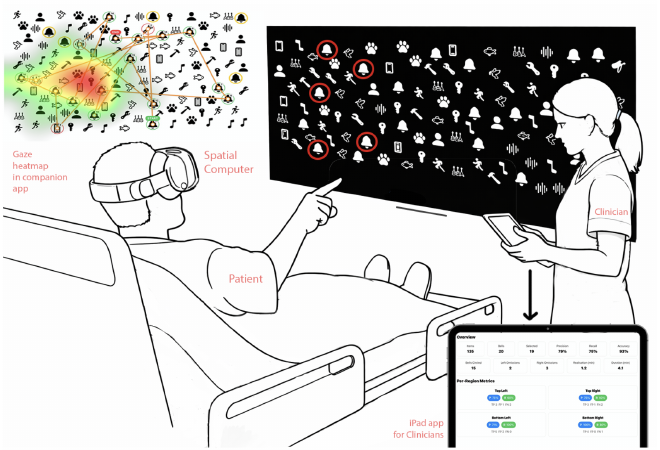
\includegraphics[width=0.85\linewidth]{bellstrace.png}
    \caption{BellsTrace}
    \label{fig:bellstrace}
\end{figure}
Unilateral spatial neglect (USN) is a common and disabling consequence of stroke, yet it is still assessed mainly with the paper-and-pencil Bell's Test, which is standardized but poor at capturing how neglect shows up in real, everyday scenes. Testing whether an immersive version adds anything has been held back by the lack of shared hardware that can run both kinds of test the same way. We present BellsTrace, a cross-device system that pairs a head-mounted spatial computer (Apple Vision Pro) with a clinician's tablet (iPad). The patient wears the headset and does nothing else; the clinician configures, starts, monitors, and aborts the session from the tablet. The Bell's Test runs in two media on the same device through one scoring pipeline: a standardized static field, and a VR180 field with the same targets composited over stereoscopic 180$^\circ$ video, which can be filmed once in any real environment without 3D asset authoring. From gaze and selection telemetry the pipeline produces three clinician-facing products: a per-quadrant Bell's Test report (hits, misses, false positives, precision, recall, lateralized omissions, timing), a VR180 gaze-session summary with a drift asymmetry index, and a gaze/omission heatmap with a reconstructed search path.

The paper reports three design iterations (from a free-look field, to a head-locked field, to the current hands-free, tablet-controlled version) and a demonstration on real sessions with four chronic stroke cases and four healthy controls at a community stroke-rehabilitation organization, together with a full IRB-style protocol for a powered follow-on study. Both media ran end-to-end on every patient, and cases given the same 1--5 clinician rating were separated by the continuous gaze indices.

\noindent\textbf{Participant feedback.} I designed and administered a post-session participant questionnaire (v1.0) covering prior assessments, usability, comfort, comparison with paper tests, everyday relevance, and willingness to adopt. Early responses from chronic stroke participants (one haemorrhagic, one ischaemic; both had previously done the Bell's Test and star cancellation) were encouraging: instructions, task clarity, and scene clarity were all rated 4/5; one participant rated the VR180 session \textit{better} than the paper test on four of five comparisons (easier to understand, less tiring, closer to everyday looking, preferable to repeat), would ``probably'' take it in place of a paper test, and would accept 4--6 sessions a month. Responses also surfaced design constraints: dizziness and session length were the main deterrents, and one participant with cervical-spine involvement and high spasticity reported low comfort (2/5), informing headset fit and session-length decisions for the follow-on study.

% ---
\subsection{SpatialTrace: Leveraging Spatial Computing for Objective Motor Incoordination Assessment}
\label{subsec:spatialtrace}

\noindent\textbf{Status:} First-Author Manuscript prepared for
\href{https://www.jmir.org/}{JMIR}
(\textit{Journal of Medical Internet Research}); invention disclosure filed, so technical details are generalised here pending patenting.\\

Dysmetria (overshooting or undershooting a target during movement) is a hallmark of cerebellar dysfunction after stroke and in degenerative ataxia and related neurological disorders. The current gold standard, the finger-to-nose exam, relies on the clinician's eye and experience, with inter-rater agreement (Cohen's $\kappa \approx 0.36$--$0.40$) below accepted clinical thresholds, and international working groups have called for standardized sensor-derived outcome measures. SpatialTrace is a spatial computing application that turns this bedside exam into a quantitative, repeatable assessment in passthrough mixed reality, where patients still see their own hands and surroundings. The headset captures hand movement during guided tasks, and a companion tablet app gives clinicians immediately readable results (per-task summaries, trajectory visualisations, severity indicators, and longitudinal trends) without the clinician wearing the headset.

The manuscript covers the system architecture, task design, metric definitions, data-labelling method, and a pilot evaluation. A ward pilot at Alexandra Hospital (NUHS) with 5 controls and 6 patients with cerebellar stroke or ataxia, scored by a neurologist, showed that the kinematic measures clearly separated patient tracing from control tracing and quantified tremor at millimetre scale. The study runs under NUHS IRB certification with Dr.\ Lim Jeong Hoon (Senior Consultant, Rehabilitation Medicine) as clinical champion.

% ---
\subsection{SpatialTrace Translation: Investor Deck and Funding Application with NUHS (Figure~\ref{fig:pitch})}
\label{subsec:spatialtrace-funding}

\noindent\textbf{Status:} Draft investor deck prepared for the NUHS
\textit{PULSE Programme} pitch (October 2026); funding outcome pending.\\
\begin{figure}[h]
    \centering
    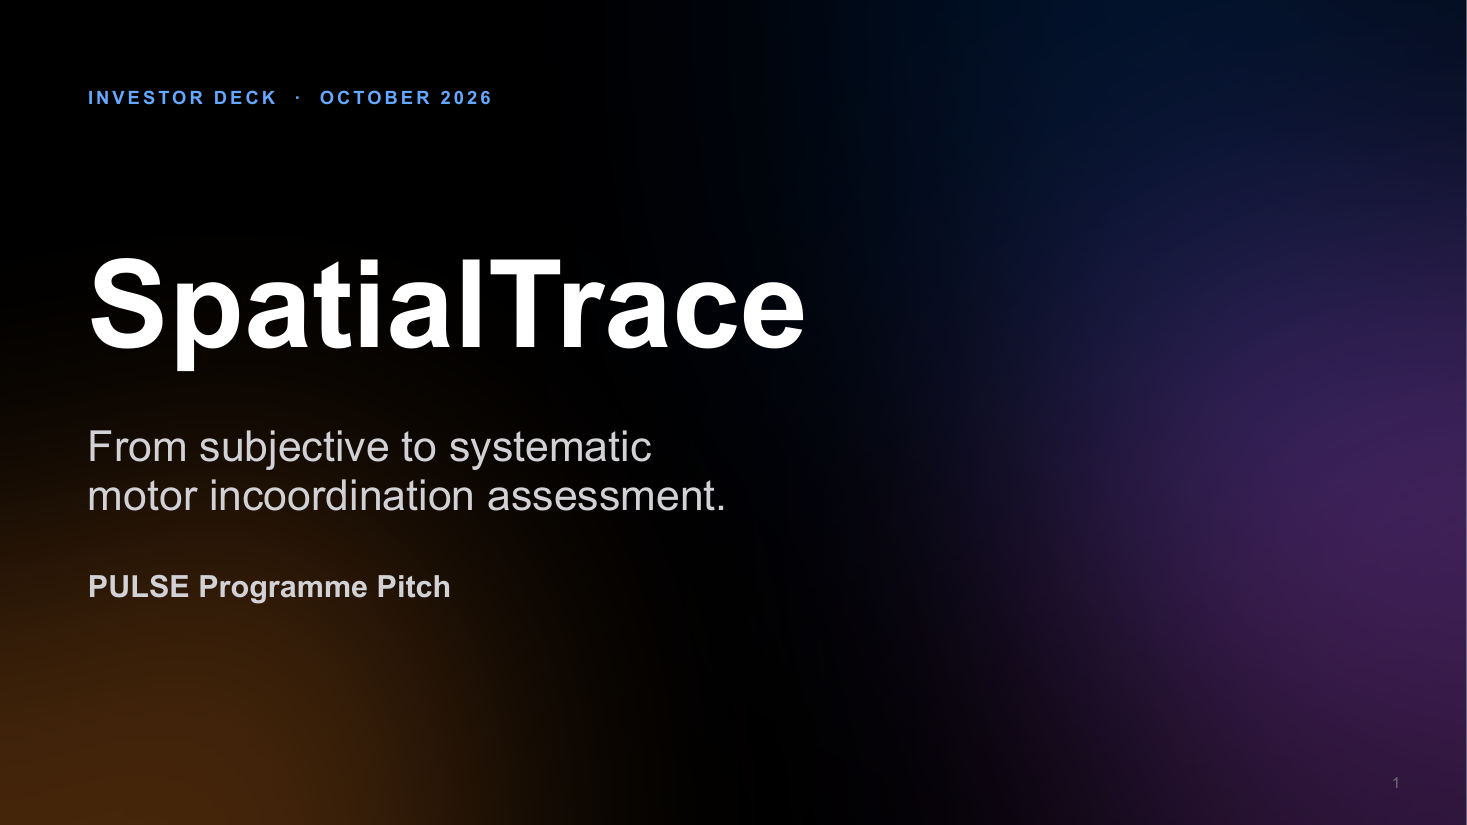
\includegraphics[width=0.6\linewidth]{spatialtrace_pitch.png}
    \caption{SpatialTrace investor deck (title slide)}
    \label{fig:pitch}
\end{figure}

To move SpatialTrace beyond a research prototype, I led the preparation of an investor deck with NUHS to seek translational funding. The deck frames the problem (coordination graded 0--4 by eye, no numbers saved per visit), the market (an estimated 130--220M people worldwide living with motor incoordination across stroke, tremor, Parkinson's, MS, and ataxia), the solution and ward-pilot evidence, a two-tier business model (clinic/hospital and at-home versions), an HSA Class~B Clinical Decision Support regulatory pathway, a phased Singapore $\rightarrow$ ASEAN $\rightarrow$ US/EMEA go-to-market plan, and an IP strategy. The ask is \textbf{SGD 78,900} over 12 months to build an 80--100-participant reference database with hand-specific norms, validate tracking accuracy against a motion-capture reference, and lock the clinical protocol, positioning the project for follow-on funding.

As customer discovery, I conducted scoping interviews and questionnaires with clinicians across primary care, neurorehabilitation, and emergency medicine. Key findings: left--right hand differences are a key metric clinicians want; quantified, trackable data matters most to GPs and rehabilitation teams who follow patients over time; and the tool should be positioned as decision support (``like an ECG'': it measures, the clinician decides).

% ---
\subsection{Vestibalance: Filling in the Data Blanks (Figure~\ref{fig:vestibalance})}
\label{subsec:vestibalance}

\noindent\textbf{Status:} Poster presented at the
\textit{KK Women's and Children's Hospital Paediatrics ACP Academic Week}
(\textit{Academic Clinical Programme}). Co-advised by Dr.\ Gabriel Lipkowitz and Muhammad Alif Bin Abu Bakar.\\
\begin{figure}[h]
    \centering
    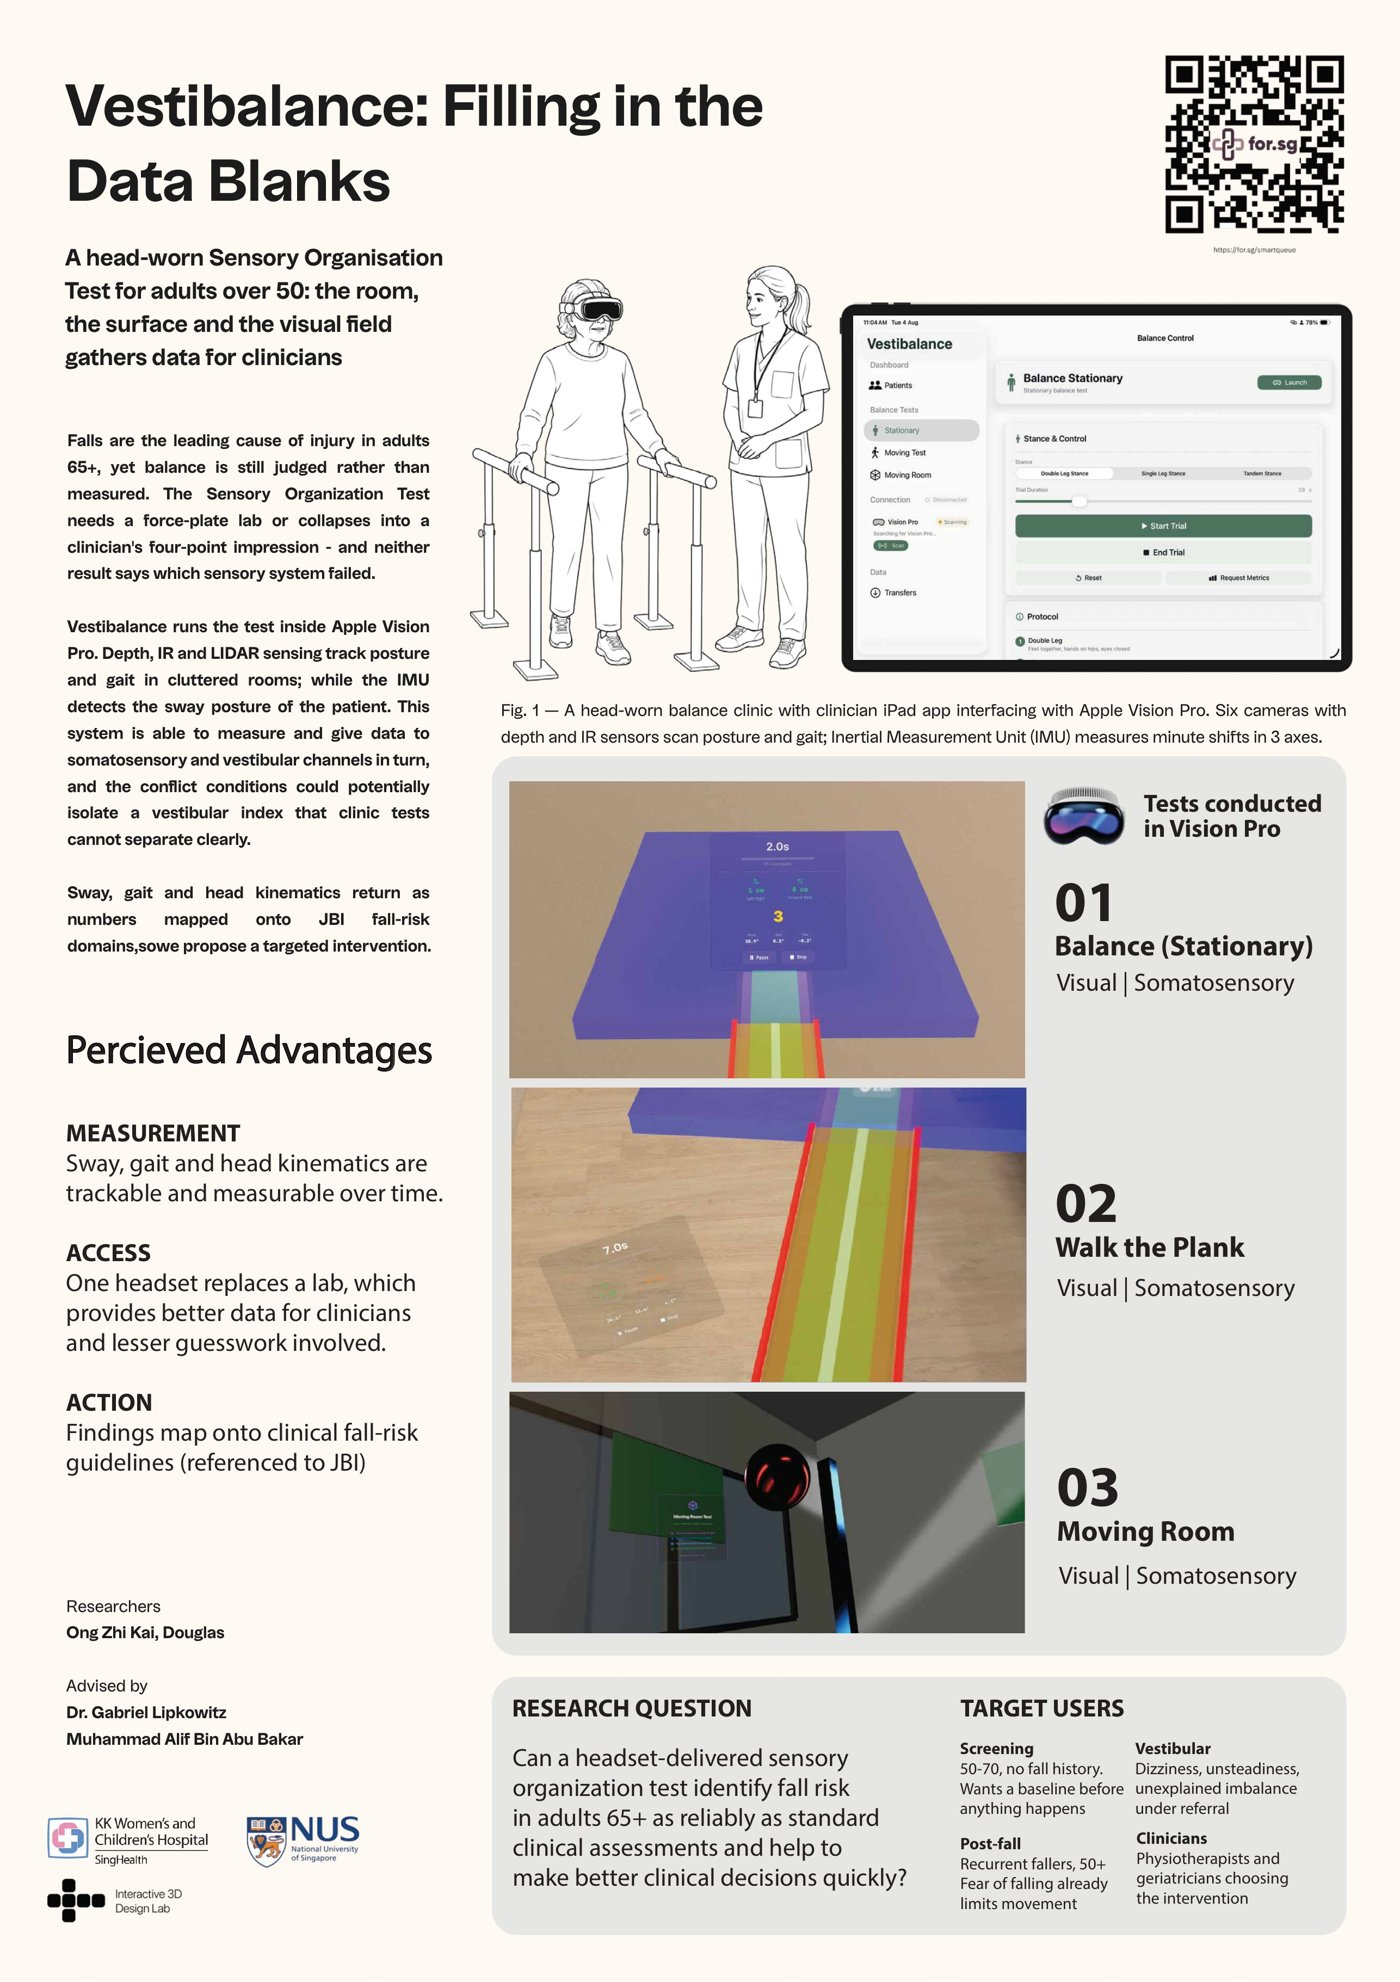
\includegraphics[width=0.48\linewidth]{vestibalance.jpg}
    \caption{Vestibalance poster}
    \label{fig:vestibalance}
\end{figure}

Falls are the leading cause of injury in adults aged 65 and over, yet balance is still judged rather than measured. The Sensory Organization Test needs a force-plate lab or collapses into a clinician's four-point impression, and neither result says which sensory system failed. Vestibalance runs a head-worn Sensory Organization Test inside Apple Vision Pro, with a clinician iPad app controlling the session. Depth, IR, and LiDAR sensing track posture and gait in cluttered rooms while the IMU detects postural sway; three tests (\textit{Balance (Stationary)}, \textit{Walk the Plank}, and \textit{Moving Room}) manipulate visual and somatosensory input in turn, so the conflict conditions could isolate a vestibular index that clinic tests cannot separate clearly. Sway, gait, and head kinematics are returned as numbers mapped onto JBI fall-risk domains to guide targeted intervention. The research question is whether a headset-delivered Sensory Organization Test can identify fall risk in adults 65+ as reliably as standard clinical assessments and support faster clinical decisions. Target users include adults 50--70 seeking a baseline, recurrent fallers, people under vestibular referral, and the physiotherapists and geriatricians choosing the intervention.

% ---------------------------------------------------------------------------
\section{Academic Service}
% ---------------------------------------------------------------------------

\begin{itemize}[leftmargin=1.5em]
    \item Served as Student Volunteer at
          \href{https://dis.acm.org/2026/}{ACM DIS 2026}, Singapore
          (\textit{ACM Designing Interactive Systems Conference})
\end{itemize}

% ---------------------------------------------------------------------------
\section{Teaching and Mentoring}
% ---------------------------------------------------------------------------

\begin{itemize}[leftmargin=1.5em]
    \item Student Mentor at \textit{SpatialHack AI 2026}: guided participant teams on spatial computing concepts, scoping, and prototyping of their hackathon projects
\end{itemize}

% ---------------------------------------------------------------------------
\section{Courses Taken}
% ---------------------------------------------------------------------------

\begin{footnotesize}
\noindent
\begin{minipage}[t]{0.46\textwidth}
  \textbf{2026/2027 Semester 1}\\[0.4em]
  \begin{tabular}{@{}p{1.3cm}p{4.2cm}r@{}}
  \toprule
  \textbf{Code} & \textbf{Description} & \textbf{Units} \\
  \midrule
  \textcolor{red}{[CODE]} & \textcolor{red}{[Course title]} & \textcolor{red}{[x.00]} \\
  \textcolor{red}{[CODE]} & \textcolor{red}{[Course title]} & \textcolor{red}{[x.00]} \\
  \bottomrule
  \end{tabular}
\end{minipage}
\end{footnotesize}

% ---------------------------------------------------------------------------
\section{Other Activities}
% ---------------------------------------------------------------------------

\begin{itemize}[leftmargin=1.5em]
    \item Field user studies with chronic stroke survivors at a community stroke-rehabilitation organization (BellsTrace), including design and administration of a post-session participant questionnaire
    \item Ward pilot at Alexandra Hospital, NUHS (SpatialTrace)
    \item Clinician customer-discovery interviews in primary care, neurorehabilitation, and emergency medicine (SpatialTrace)
    \item Investor pitch preparation for the NUHS PULSE Programme (SpatialTrace)
    \item Poster presentation at KKH Paediatrics ACP Academic Week (Vestibalance)
\end{itemize}

% ---------------------------------------------------------------------------
\section{Self-Assessment}
% ---------------------------------------------------------------------------

I consider this semester productive and on track. My work has converged on a coherent research direction, cross-device, clinician-in-the-loop spatial computing for objective neurological assessment, and I have applied a shared architecture (patient-worn spatial computer, clinician tablet, one telemetry pipeline) across three clinical problems: spatial neglect (BellsTrace), motor incoordination (SpatialTrace), and balance and fall risk (Vestibalance). Each project has reached real patients or clinicians rather than remaining a lab prototype.

\begin{itemize}[leftmargin=1.5em]
    \item \textbf{Research output:} one first-author paper submitted (CHI 2027), one first-author journal manuscript prepared (JMIR), and one poster presented (KKH ACP Academic Week).
    \item \textbf{Clinical engagement:} I have built working relationships with clinical partners at NUHS, KKH, and a community stroke-rehabilitation organization, and gained experience with IRB processes and running studies with vulnerable populations.
    \item \textbf{Translation:} I developed skills beyond HCI research (market sizing, regulatory pathways, IP strategy, and pitching) through the SpatialTrace funding effort.
    \item \textbf{Areas to improve:} my pilot samples are small and not statistically powered; next semester I need to prioritise powered, pre-registered studies and stronger quantitative analysis, and balance the number of parallel projects against depth.
\end{itemize}

% ---------------------------------------------------------------------------
\section{Other Comments}
% ---------------------------------------------------------------------------

\textbf{Achievements.}
\begin{itemize}[leftmargin=1.5em]
    \item Submitted BellsTrace as first author to ACM CHI 2027, with real-world sessions on chronic stroke survivors.
    \item Completed a ward pilot of SpatialTrace at Alexandra Hospital and filed an invention disclosure.
    \item Prepared an investor deck with NUHS seeking SGD 78,900 to build the SpatialTrace reference database.
    \item Presented Vestibalance at the KKH Paediatrics ACP Academic Week.
    \item Served the community as Student Volunteer at ACM DIS 2026 and Student Mentor at SpatialHack AI 2026.
\end{itemize}

\textbf{Problems encountered.}
\begin{itemize}[leftmargin=1.5em]
    \item \textit{Participant comfort and accessibility:} stroke survivors vary widely in impairment (aphasia, limb weakness, spasticity, cervical-spine involvement). Headset comfort, dizziness, and session length emerged as the main barriers in participant feedback, requiring shorter sessions and a hands-free patient interface.
    \item \textit{Recruitment and sample size:} access to patients is limited and slow, so current results show technical feasibility rather than diagnostic validity; larger multi-site studies are planned.
    \item \textit{Metric validity:} the current VR180 drift index is computed per eye rather than per hemispace, and needs refinement before it can be read as a neglect index.
    \item \textit{IP and publication timing:} SpatialTrace publication must be sequenced around the patenting process, which limits how much detail can be shared in the meantime.
\end{itemize}

\end{document}
